%
% sinspline.tex
%
% (c) 2024 Prof Dr Andreas Müller
%
\begin{figure}
\centering
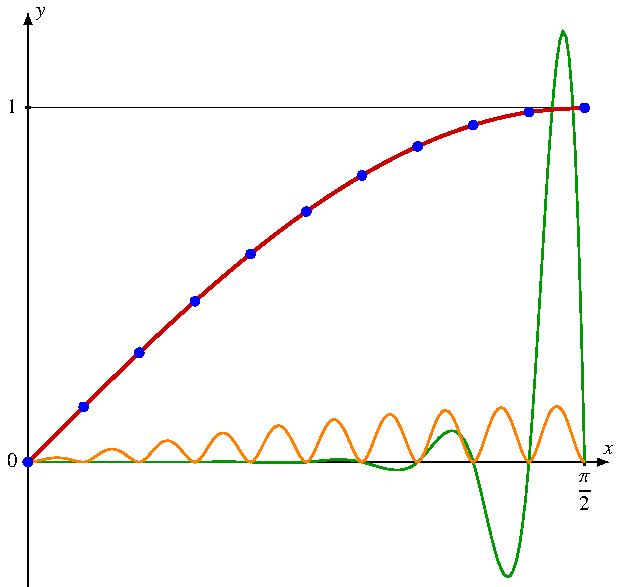
\includegraphics{chapters/030-nichtdiff/images/sinspline.pdf}
\caption{Approximation der Sinus-Funktion mit einer
Spline-Interpolationsfunktion mit nur 11 Stützstellen
(Beispiel~\ref{buch:nichtdiff:splines:bsp:sinspline}).
Der Unterschied zwischen $\sin x$ und $y(x)$ ist kaum erkennbar,
die grüne Kurve zeigt die Differenz $1000\cdot(\sin x - y(x))$.
Der Fehler der Spline-Interpolationsfunktion wird bestimmt durch
die Genauigkeit, mit der die Steigungen durch das Gleichungssystem
\ref{buch:nichtdiff:splines:eqn:gleichungssystem} geschätzt wird.
Die orange Kurve zeigt den $10^5$-fach überhöhten Fehler, wenn die
Steigungen mit $\cos x_k$ exakt bestimmt werden.
\label{buch:nichtdiff:splines:fig:sinspline}}
\end{figure}
